% 
% Annual Cognitive Science Conference
% Sample LaTeX Paper -- Proceedings Format
% 

% Original : Ashwin Ram (ashwin@cc.gatech.edu)       04/01/1994
% Modified : Johanna Moore (jmoore@cs.pitt.edu)      03/17/1995
% Modified : David Noelle (noelle@ucsd.edu)          03/15/1996
% Modified : Pat Langley (langley@cs.stanford.edu)   01/26/1997
% Latex2e corrections by Ramin Charles Nakisa        01/28/1997 
% Modified : Tina Eliassi-Rad (eliassi@cs.wisc.edu)  01/31/1998
% Modified : Trisha Yannuzzi (trisha@ircs.upenn.edu) 12/28/1999 (in process)
% Modified : Mary Ellen Foster (M.E.Foster@ed.ac.uk) 12/11/2000
% Modified : Ken Forbus                              01/23/2004
% Modified : Eli M. Silk (esilk@pitt.edu)            05/24/2005
% Modified : Niels Taatgen (taatgen@cmu.edu)         10/24/2006
% Modified : David Noelle (dnoelle@ucmerced.edu)     11/19/2014
% Modified : Roger Levy (rplevy@mit.edu)             12/31/2018



%% Change "letterpaper" in the following line to "a4paper" if you must.

\documentclass[10pt,letterpaper]{article}

\usepackage{cogsci}

%\cogscifinalcopy % Uncomment this line for the final submission 


\usepackage{pslatex}
\usepackage{apacite}
\usepackage{graphicx}
\usepackage[colorinlistoftodos]{todonotes}
\usepackage{float} % Roger Levy added this and changed figure/table
                   % placement to [H] for conformity to Word template,
                   % though floating tables and figures to top is
				   % still generally recommended!
\usepackage{amsmath}

%\usepackage[none]{hyphenat} % Sometimes it can be useful to turn off
%hyphenation for purposes such as spell checking of the resulting
%PDF.  Uncomment this block to turn off hyphenation.

\definecolor{Orange}{RGB}{255,140,0}
\newcommand{\ek}[1]{\textcolor{Orange}{[ek: #1]}} 

\definecolor{Purple}{RGB}{255,10,140}
\newcommand{\jd}[1]{\textcolor{Purple}{[jd: #1]}} 


%\setlength\titlebox{4.5cm}
% You can expand the titlebox if you need extra space
% to show all the authors. Please do not make the titlebox
% smaller than 4.5cm (the original size).
%%If you do, we reserve the right to require you to change it back in
%%the camera-ready version, which could interfere with the timely
%%appearance of your paper in the Proceedings.



\title{Production Expectations Modulate Contrastive Inference}
 
\author{{\large \bf Elisa Kreiss (ekreiss@stanford.edu)} \\
  Department of Linguistics, 460 Jane Stanford Way \\
  Stanford, CA 94305 USA
  \AND {\large \bf Judith Degen (jdegen@stanford.edu)} \\
  Department of Linguistics, 460 Jane Stanford Way \\
  Stanford, CA 94305 USA}


\begin{document}

\maketitle

\begin{abstract}
Include no author information in the initial submission, to facilitate
blind review.  The abstract should be one paragraph, indented 1/8~inch on both sides,
in 9~point font with single spacing. The heading ``{\bf Abstract}''
should be 10~point, bold, centered, with one line of space below
it. This one-paragraph abstract section is required only for standard
six page proceedings papers. Following the abstract should be a blank
line, followed by the header ``{\bf Keywords:}'' and a list of
descriptive keywords separated by semicolons, all in 9~point font, as
shown below.

\textbf{Keywords:} 
add your choice of indexing terms or keywords; kindly use a
semicolon; between each term
\end{abstract}

\section{Introduction}

One of the most interesting features of language is its flexibility. To refer to one single object a speaker can choose an utterance out of an indefinite set of possible referring expressions. \textit{The banana}, \textit{the yellow banana}, \textit{the yellow, curvy fruit-thingy} for example are all possible utterances that can refer to the same object. At the same time, the same utterance -- e.g., \emph{banana} -- can be used to refer to different kinds of objects. But this flexibility poses a challenge for the listener, who needs to pragmatically infer the speaker's intention. Consequently, trying to understand how a listener processes these utterances and what affects their interpretation has become a central question in psycholinguistic research. 
% In comprehension all of these utterances still need to be interpreted as describing this same object in this particular context in Figure~\ref{example-context}. Consequently, trying to understand how a listener processes these utterances and what affects their interpretation has become a central question in psycholinguistic research. \jd{too nitty-gritty. get rid of the figure (or replace it with a version of fig 4 that just has the display, without the audio stim and time window info), just say "are all possible utterances that can be used for the same object. At the same time, the same utterance -- e.g., \emph{banana} -- can be used to refer to different kinds of objects". Raise the issues independently of the figures: this flexibility poses a challenge for listeners, who need to pragmatically infer the speaker's intention.}

One of the most fundamental findings is that listeners process utterances incrementally, i.e., new information is incorporated into the interpretation of the utterance as soon as it becomes available \cite{Eberhard:1995}. For instance, eye-tracking experiments have shown that if a listener hears the incomplete utterance \textit{the yellow} in a display like Figure~\ref{example-context}a, they fixate the yellow objects in the display even before they hear the disambiguating noun \textit{banana} and \ek{arrive at} the final referent \ek{cite}.

But listeners go beyond the information contained in the signal itself; they also take into account contextual information and specifically the nature of other possible referents to draw rapid pragmatic inferences about the speaker's intention \ek{cite}. One of those inferences is called the ``contrastive inference'' \cite{Sedivy:1999}. Consider the context in Figure~\ref{example-context}a that shows a yellow an orange banana, a yellow corncob and some other distractor item. When a listener is asked to \textit{pick out the yellow...}, there are two eligible objects to choose from: the yellow banana and the yellow corncob. \cite{Sedivy:1999, Sedivy:2003} shows that when there is a contrast to one of the objects (here, another banana), listeners rather fixate the yellow banana than the corncob, suggesting that there is a preference for the banana interpretation \cite{Eberhard:1995}. 

Originally, this effect has been shown with size adjectives in eyetracking experiments \cite{Sedivy:1999} and has since been replicated reliably, especially in the scalar adjective domain \ek{cite}. However the effect seems to be less stable with color adjectives \cite{Sedivy:2003}. \citeA{Sedivy:2003} reports that the contrastive inference arises in contexts where the target object has a ``predictable'' color (such as the yellow banana in Figure~\ref{example-context}a) but not when it is replaced by an object with an ``unpredictable'' color like a cup. 
They suggest that those objects differ in how likely a speaker is to produce the color modifier for the object in isolation, i.e., in the absence of a contrast, a yellow banana is usually just called a \textit{banana} while a yellow cup is still sometimes called a \textit{yellow cup}.

% \jd{this is a weird example because it moves the focus towards prediction of lexical material even though what we're interested in is prediction of the speaker's intended referent. use this space instead to already introduce the contrastive inference. use a display akin to the sedivy 2003 color-diagnostic displays so you can introduce the contrastive inference using color terms and then segue into the issue that contrastive inferences variably do or don't arise, especially within the color term domain (but also mention size). then discuss the different approaches that have been taken to explain why contrastive inferences do/don't arise and introduce your own, RSA-based one that ties the disparate findings together}

\begin{figure}
	\begin{center}
		\includegraphics[width=.475\textwidth]{graphs/Sedivy2003-contexts.pdf}
	\end{center}
\caption{This is a figure. \ek{UPDATE FIGURE! This should show a ttp context left and a tap context on the right}} 
\label{example-context}
\end{figure}



% \begin{figure}
% 	\begin{center}
% 		\includegraphics[width=.475\textwidth]{graphs/example-context.pdf}
% 	\end{center}
% \caption{This is a figure. \ek{what figure here? Should I already include "Click on the yellow..." above and a mouse pointing to the yellow banana? This would immediately prepare for the paradigm on the first glance.}} 
% \label{example-context}
% \end{figure}


Since then inferences have been shown to be modulated by multiple factors, including adjective semantics \ek{cite}, property salience \ek{cite}, speaker reliability \ek{cite}, and expectations of informativity \ek{cite Sedivy 2003}.\jd{say a sentence about each of these, to introduce what you mean by all these different terms, but also to give a reader a sense for how much of an unsatisfying laundry list of features this comprises.}

\jd{"We provide a novel account of contrastive inferences that has the potential to unify all the above properties by reducing them to listeners' expectations about the speaker's contextual probability of producing the pre-nominal adjective. We couch this account within the Rational Speech Act framework... etc, leading into the next paragraph"}

Following recent research highlighting the importance of the listener’s generative model of the speaker in generating pragmatic inferences \ek{cite}, we propose the Rational-Speech Act (RSA) framework \ek{cite} as a new way to think about contrastive inference incrementally. In this framework, the listener reasons about a speaker's possible utterances, therefore giving the speaker model a central role in the predictions. It provides a way to quantitatively assess which predictions a listener with prior beliefs and expectations about the speaker \textit{should} make. This shifts the focus away from specific cognitive and linguistic factors that influence contrastive inference onto listener's production expectations (and their prior beliefs). 
\jd{nice}

In this paper we will first show on qualitative examples how the RSA account can make the same predictions about the basic contrast effect as for instance the default description \cite{Grodner:2005,Sedivy:1999,Sedivy:2003} or the contrastive-adjective-function account \ek{cite}. We will then show new predictions about factors affecting contrastive inferences. To test the model, we report a production study to get modifier probability estimates.we then collect the data we want to model in a comprehension experiment using an incremental decision task (which will also serve as a proof of concept that contrastive inferences can be elicited in offline tasks); then model evaluation.

% \jd{interest: what information listeners recruit in drawing pragmatic inferences (in this case contrastive ones) online}

% \section{Related Work}
% \jd{i know this kind of section is common at acl type conferences, but at cogsci it's not. leave out this section and merge the relevant stuff into the intro and into the model section}

% Since the introduction of the paradigm in \ek{Sedivy 1999}, the contrastive inference effect has been replicated especially in the size adjective domain \ek{cite} and has been shown to be modulated by multiple factors. \ek{CI is shown to be modulated by multiple factors, including adjective semantics [2], property salience [3], speaker reliability [4,5], and expectations of informativity [6] \ek{cite}.} 

% These accounts which investigate specific factors that give rise to a contrastive inference indirectly put more or less relevance onto the speaker.
% \ek{Sedivy 1999} for instance only considers a very limited speaker model. In this account, a contrastive inference arises when the modifier is not a component of the object's \textit{default description}. In other words, since \textit{tall} is added to the default description \textit{the glass}, the adjective elicits a contrastive inference in the listener. It therefore only assumes speaker considerations as to the creation of the default descriptions for objects and is completely independent of the context the target is presented in. \ek{explain color case here}

% \ek{cite rubio fernandez} gives the speaker a more central role. In this account, the production probabilities of this more involved speaker directly affect the size of the contrastive inference. It therefore predicts that contrastive inference is not binary, but can occur in different strengths. While this account considers listeners' reasoning not only about the target but also about the competitor, the speaker model is still restricted to target considerations only. \ek{write this better}

% In this work, we use the RSA framework to quantitatively assess how a highly pragmatic listener with a generative speaker model should draw contrastive inferences. \ek{cite 7, 8} \ek{explain general idea of RSA}


\section{Accounts of contrastive inference \ek{Model section}}

\ek{"Likelihood" and "probability" are all scrambled up here. Don't forget to fix that!}

In the literature, different factors have been considered to give rise to contrastive inference which indirectly put more or less relevance onto the speaker. 

\citeA{Sedivy:1999} for instance only considers a very limited speaker model. In this account, a contrastive inference arises when the modifier is not a component of the object's \textit{default description}. In other words, since \textit{yellow} is added to the default description \textit{the banana}, the adjective elicits a contrastive inference in the listener. It therefore only assumes speaker considerations as to the creation of the default descriptions for objects and is completely independent of the context the target is presented in.

\ek{cite rubio fernandez} gives the speaker a more central role. In this account, the production probabilities of this more involved speaker directly affect the size of the contrastive inference. It therefore predicts that contrastive inference is not binary, but can occur in different strengths. While this account considers listeners' reasoning not only about the target but also about the competitor, the speaker model is still restricted to target considerations only. \ek{write this better}

A Rational-Speech Act account gives the speaker a central role in the predictions, since the listener directly reasons about the speaker's possible utterances $u$ for each object $r$ in the display $C$. 

\begin{equation}
	P_{L_1}(r|u,C) = \frac{P_{S_0}(u|r,C) * P(r|C)}{\Sigma \space P_{S_0}(u|r_{i},C) * P(r_{i}|C)}
\label{eq-prior}
\end{equation}

For now we will make the simplifying assumption that listeners have a uniform prior over all objects in the display. Then the RSA model predicts a direct relationship between the production probabilities and the listener's distribution over possible referents. So far in the literature, RSA has been mainly applied to the analysis of full utterances. To receive RSA predictions after an incomplete reference such as \textit{the yellow...}, $P_{S_0}$ is simply the underlying probability of color mention for each referent in the display. 

To understand the qualitative predictions of the RSA account, we will first consider the context in Figure~\ref{example-context}a and so far the speaker message available to the listener is \textit{Click on the yellow...}. The pragmatic listener $P_{L_1}$ will now consider how likely a speaker is to include the modifier \textbf{yellow} in their referring expression \textbf{for each object in the display}. Since only the target (yellow banana) and competitor (corncob) are yellow, we will assume that the production probabilities of \textit{yellow} for other objects in the display are 0. 

If the contrasting banana is absent, speakers are unlikely to include the color modifier when referring to the target banana \ek{number} and they are equally unlikely to do so for its competitor, the corncob \ek{number}. The pragmatic listener will therefore not be able to prefer one potential referent over the other.

The presence of the orange banana will not affect the listener's expectations about modifier production for the competitor (corncob). However, since the modifier is now necessary for a unique identification, the speaker is much more likely to use the modifier \ek{number}. Here, the pragmatic listener then predicts the yellow banana to be the more likely target over the competitor \ek{number vs number}, and therefore predicting the generally reported case of contrastive inference.

In contrast to previous accounts of contrastive inference, the prediction on whether a ``contrastive inference'' \ek{this term here is flaky; see "thought" below} arises is not only dependent on the choice of the target object but also the competitor. This raises the questions what happens if we change the modifier production probabilities for the competitor. \ek{Westerbeek} showed that speakers are more likely to include the color modifier for objects in isolation when they appear in an typical color. This would predict that the yellow strawberry in Figure~\ref{example-context}b would receive a higher modifier production probability than the corncob competitor in Figure~\ref{example-context}a. 

\ek{Now compare how this changes things.}

The elicited production probabilities for the example objects in Figure~\ref{example-context} are displayed in Table\ek{table}.

% This strong integration of the context makes it also to a highly pragmatic account. 
% Equation (explain incrementality), table of production probabilities, explain how the two figure predictions differ

\ek{thought: the term contrastive inference is so confusing. Because there is a contrastive inference in the tan-tap case, but it's not simply: "Is there a target preference in the contrast present case", but is there a target preference compared to the non-contrast condition. I.e., if you define the contrastive inference as the preference of the target over the competitor when the contrast is present, there is no contrastive inference in the tap condition. But if you define it as the change in preference from contrast absent to contrast present, then there still is a contrastive inference. This issue makes describing the "occurrence of contrastive inference" difficult here -- maybe we should address that?}


\jd{introduce the two example contexts ttp and tap first and what different accounts predict for them (all except for RSA make the same prediction, namely the inference should arise). postulate production values for the RSA speaker model (take them from the empirically elicited values so people already have the right numbers in their head as they're reading)}

\ek{RSA model here, formula; how we define the prior,...
how is it incremental? NEW
example predictions;
talk about Westerbeek study}

To investigate when a listener with a generative speaker model should draw a contrastive inference, we need to elicit how likely a listener can expect a modified over an unmodified referring expression for each object in the display. To evaluate the performance of the model and to gain information about the prior of the objects, we need comprehension data that informs us which object is considered the most likely target referent.


\section{Experiment 1: Modifier Production in an Interactive Reference Game}

To investigate whether production probabilities affect listeners' contrastive inferences, we need to manipulate how likely a listener is to observe a modified utterance for each object in the display.\jd{this first sentence should be in the previous paragraph. here just say "Exp.~1 was aimed at obtainining modifier production probabilities for all the displays ultimately used in the contrastive inference  experiment (Exp.~2). We elicited these probabilities in a free production interactive reference game."} Our main assumption is that the typicality of a color for an object will affect these modifier production probabilities. When the object is in isolation for instance, a listener should expect the speaker to call a yellow banana simply \textit{the banana}, but a blue banana \textit{the blue banana}. In this production experiment, we tested this hypothesis and empirically elicited the proportion of color modifier mention for the target and competitor. The results are taken as the basis of what production probabilities a listener can expect to observe.


\subsection{Participants}
\jd{just flagging this section as one that can be radically shortened if you run out of space}
We recruited 282 participants over Amazon Mechanical Turk, who were randomly matched to form one listener-speaker chat pair (i.e., 141 pairs in total). 
The estimated time for completion was 10 to 12 minutes and each participant was paid \$2.30. We restricted participation to workers with IP addresses in the US and an approval rate of previous work above 97\%.

Exclusions were performed on the 141 speakers, since they provided the utterances. Participants were excluded when they participated multiple times in the experiment (1 participant; 139 pairs remaining) and when they did not use a noun from the display in at least half of the cases (27 participants; 112 pairs remaining). These participants clearly misunderstood the task, using expressions such as \textit{yellow monkey} instead of \textit{yellow banana}, or \textit{should be yellow, must have teeth to eat} for \textit{corn}. All speakers indicated that their native language was English.


\subsection{Material} \label{Material}
Each context included four items, as displayed in \ek{Figure}. The pool of items consisted of 10 types (banana, broccoli, carrot, corn, egg, lettuce, pumpkin, strawberry, swan, tomato), each of which could occur in a typical or atypical color. For example, the broccoli could occur in its typical color green or in the atypical color red. The resulting pool contains 20 items, 10 of which are atypically colored. The number of colors is carefully counterbalanced such as each color occurs twice as a typical and twice as an atypical instance. All items were carefully normed for color-diagnosticity \ek{Tanaka Presnell}, typicality and nameability.


\subsection{Design}
The contexts varied in the typicality of the target, the typicality of the competitor and the presence of a contrast, resulting in eight conditions. For the critical trials, each participant saw four randomly created contexts from each of these eight conditions. In each condition we are interested in the modifier production probabilities for the target and the competitor, which is why in half of the trials when a contrast was present, the target was marked as the item to be communicated and in the other half, the competitor was marked. However when there is no contrast present, this distinction is irrelevant. For example, when target and competitor are both (a)typical, it is irrelevant, which is underlyingly coded as the target. Similarly when the modifier production probability for a typical target in context with an atypical competitor is the same as the probability for a typical competitor in a context with an atypical target. 
The fillers were eight randomly created contexts where the contrast was the item to be communicated and 20 randomly created contexts where the distractor was the item to be communicated.
Overall, each participant saw 60 different contexts (32 critical trials) in a completely randomized order.


\subsection{Procedure}
Participants were randomly paired up and each was randomly assigned either to the role of a speaker or listener. They could communicate freely through a real-time multi-player interface similar to \ek{Hawkins (2015)}. The speaker was instructed to communicate a target object out of a four-object context to the listener. The target could be identified by a green border surrounding it. The speaker and the listener saw the same set of objects but in a randomized order to avoid trivial position-based references such as ``the left one''. After the listener clicked on the presumed target, both the speaker and listener received feedback about whether the right object had been selected.

\begin{figure}
	\begin{center}
		\includegraphics[width=.475\textwidth]{graphs/prod-design.pdf}
	\end{center}
\caption{This is a figure. \ek{make text bigger in figure}} 
\label{prod-results}
\end{figure}


\subsection{Results}
\ek{only selected items with correct selection}
Figure~\ref{prod-results} shows the probability of color modifier mention for the target and competitor in each condition\footnote{Note that some data is duplicated in the conditions where the contrast is absent (\ek{see section...for explanation}). In the conditions where target and competitor are both (a)typical, the modifier probabilities are created by the same data. The underlying data is also identical in the two conditions where one of the items is (a)typical.}. 

\begin{figure}
	\begin{center}
		\includegraphics[width=.45\textwidth]{graphs/prod-bycond-paper.pdf}
	\end{center}
\caption{This is a figure. \ek{make text bigger in figure}} 
\label{prod-results}
\end{figure}

When a contrast to the target is present (e.g., another banana), a speaker needs to include the color modifier to fully disambiguate the two items (see the upper row in Figure~\ref{prod-results}). When the typicality of the target is atypical, this is completely borne out in the data. However if the target is typical, participants sometimes also used the unmodified utterance. \ek{refer to speculations about the reason for this in discussion} 

When the contrast is absent (see the lower row in Figure~\ref{prod-results}), speakers were more likely to include a color modifier when referring to an atypical target than a typical one \ek{stats?}.

Independent of contrast, speakers were more likely to include the color modifier for an atypical color competitor over a typical one \ek{stats?}.

The results of this production experiment show that the probability of a speaker's modifier use is modulated by the color typicality of the item and the presence of a contrast. Our experiment therefore manipulates the modifier production probabilities a listener can expect in different contexts.


\section{Comprehension Experiment: An Incremental Decision Task}
To investigate which objects listeners consider to be the most likely target after observing the color adjective, we conducted an incremental decision task. \ek{...}


\subsection{Participants}
We recruited 239 participants over Amazon's Mechanical Turk, 121 of which saw atypical color competitors and 118 saw typical color competitors in the critical trials. The study took on average 7 minutes and each of them were paid \$1.80 for their participation. We restricted participation to workers with IP addresses in the US and an approval rate of previous work above 97\%.

We excluded participants who did the Hit multiple times (1) who indicated that they did the Hit incorrectly or were confused (13), who indicated that they had a native language other than English (6), and who gave more then 20\% erroneous responses (7). An erroneous response is defined as a click to a non-target object after observing the fully disambiguating noun, i.e., participants are excluded who selected the wrong final object more than 11 times. Overall, we excluded 27 people, which is 11\% of the subjects. 211 participants remain, 108 of which were in the atypical competitor and 103 were in the typical competitor condition. 


\subsection{Material}
The item pool is the same as described in the production study.


\subsection{Design}
\ek{clarify what is within and between-subject manipulation with rationale}

Participants completed 55 trials in total, 20 of which were critical trials and 35 were fillers. The contexts varied for each participant with respect to the presence of a contrast and the target's color typicality (within-subject manipulation). Participants were randomly assigned to see either typical or atypical competitors on critical trials (between-subject manipulation). All critical trials included color modified utterances. To avoid that participants learn that the color modifier is always part of the referring expression, we need filler trials with unmodified referring expression. Another confound could be that participants can derive the target already from the context without seeing a referring expression, since the target is the only object that shares its color and type features with other objects in the display. The filler trials therefore needed to introduce primarily unmodified referring expressions that target other objects in the display. The exact trial structure is summarized in table \ref{tab:trialstructure}.


\subsection{Procedure}
This experiment is a one-player adaptation of the production study explained above and follows the design of an incremental decision task \ek{cite Qing}. 

\begin{figure}
	\begin{center}
		\includegraphics[width=.4\textwidth]{graphs/IDT-design.pdf}
	\end{center}
\caption{This is a figure.} 
\label{prod-results}
\end{figure}

All participant were assigned the role of the listener, which means that they needed to identify which object was the target given a referring expression placed above the context. Crucially, the referring expression was only gradually revealed and participants had to choose an object each time. The choices had to be made prior any information about the target (i.e, after observing "Click on the"), after observing an adjective ("Click on the yellow") and after observing the full referring expression with the disambiguating noun ("Click on the yellow banana!"). The selections a listener makes before receiving any information about the target, inform us about potential priors they might have. The critical selections are the clicks after observing the adjective but before the disambiguating noun, since they will inform us about the inferences participants seem to draw from observing the adjective. We also collected the clicks after the fully disambiguating noun was presented, which functioned as attention checks in the analysis. 

To center the position of the mouse after each selection, a button appeared in the center of the grid which had to be clicked to reveal the next word or to advance to the next trial. 

\begin{table}
	\begin{center} 
	\caption{Overview of the trial structure for the comprehension study.} 
	\label{tab:trialstructure}
	\vskip 0.12in
	\begin{tabular}{llll} 
	\hline
	\textbf{trial type} & \textbf{number} & \textbf{utterance} & \textbf{referent} \\
	\hline
	critical  & 20     & modified       & target                \\
	filler    & 5      & unmodified     & competitor (typical)  \\
	filler    & 5      & modified       & competitor (atypical) \\
	filler    & 5      & modified       & contrast              \\
	filler    & 20     & unmodified     & distractor (typical)  \\
	\hline
	\end{tabular} 
	\end{center} 
	\end{table}

Before participants proceeded to the main trials, they had to complete four practice trials constructed from the speaker perspective. In the speaker role, they saw contexts with four non-color diagnostic objects, one of which was marked as the target by a green border surrounding it. They were then asked to refer to the object such that a second player could identify it. The practice trials were introduced to familiarize the participants with the task.

The main trials were randomized with one restriction: Trials in which a speaker's color modifier use to refer to the target is very unlikely only occurred after the 15th trial. These were contexts where there was no contrast and either both target and color competitor were typical objects, or the target was typical while the color competitor was atypical. We introduced this restriction to minimize the risk that participants perceive the ``utterance generator'' (speaker) as unnatural.

% \subsection{Data Preprocessing and exclusion}

\subsection{Results}
Figure~\ref{compr-results} shows the proportion of clicks on the objects in the display prior observing the adjective (lighter colors) and after the adjective (darker colors), grouped by context condition. Before an adjective is observed, all items should appear equally likely to be the target, which is supported by the generally uniform distribution in all conditions. After the adjective is observed (darker colors), only the target and competitor are legible options and we predict that the presence of the contrast and the typicality of the objects will affect the listeners' object choices.

\begin{figure}
	\begin{center}
		\includegraphics[width=.475\textwidth]{graphs/compr-bycond-paper.pdf}
	\end{center}
\caption{This is a figure. \ek{make bars and text bigger}} 
\label{compr-results}
\end{figure}

When the contrast is present (upper row in Figure~\ref{compr-results}), there is a general preference for target selection over competitor selection. This preference is biggest for the case when the target is atypical and the competitor is typical and disappears for when the target is typical and the competitor is atypical. 

When the contrast is absent (lower row in Figure~\ref{compr-results}) and target and competitor differ in typicality, there is a preference for the item with the atypical color. When the two items share their typicality, the selection are approximately at the same rate. 

These results clearly show that the color typicality of the objects in the display affect the inference listeners draw about the target. We will turn to how these results correspond to the production data by considering the RSA model predictions.

\section{Model evaluation}

To assess the relationship between the modifier production probabilities and the comprehension data in the simplest way, we will assume a flat prior over all objects in the display. The probabilities to choose the target over the competitor are then simply the normalized modifier production probabilities as shown in Equation~(\ref{eq-flatprior}), where $r$ is the possible referent, $u$ the utterance and $C$ the specific context.

\begin{equation}
	P_{L_1}(r|u,C) = \frac{P_{S_0}(u|r,C)}{P_{S_0}(u|r_{target},C) + P_{S_0}(u|r_{comp},C)}
\label{eq-flatprior}
\end{equation}

Figure~\ref{model-results-flatprior} shows the model predictions (in blue) and the empirical results (in purple) for target and competitor selection after observing the adjective. 

The model predicts...

The model qualitatively predicts the patterns for the different context conditions. However, it generally predicts a stronger inference than borne out in the empirical data. \ek{which is why the correlation is so low}

\begin{figure}
	\begin{center}
		\includegraphics[width=.475\textwidth]{graphs/model-bycond-paper.pdf}
	\end{center}
\caption{This is a figure.} 
\label{model-results-flatprior}
\end{figure}

\begin{figure}
	\begin{center}
		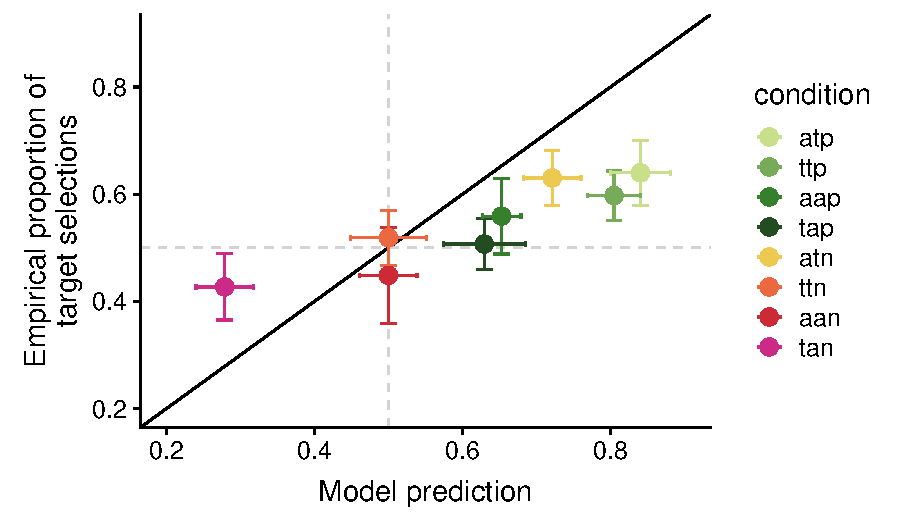
\includegraphics[width=.475\textwidth]{graphs/corr-modelflat-bycondition.pdf}
	\end{center}
\caption{This is a figure.\ek{fix condition naming}\jd{don't say "clicks to the target" but instead "target selection" on the y-axis and throughout the paper. clicks sounds clumsy. maybe also highlight the ttp and tap conditions visually if you use them as the motivating example at the beginning of the paper}} 
\label{model-results-corr-flatprior}
\end{figure}

\ek{the rsa model is a significant predictor for the comprehension data; however there are also biases: position and non-switching (see figure); in fact if we add these predictors to the model, they also become significant. In the new plots, we can see that (when the position is equal), whatever was previously clicked highly affects the outcome. Now the model underpredicts the target clicks in most conditions. The reverse is true if the competitor was clicked previously. This is something where the eyetracking data will provide more information since we expect the switching cost to be lower.}

\begin{figure}
	\begin{center}
		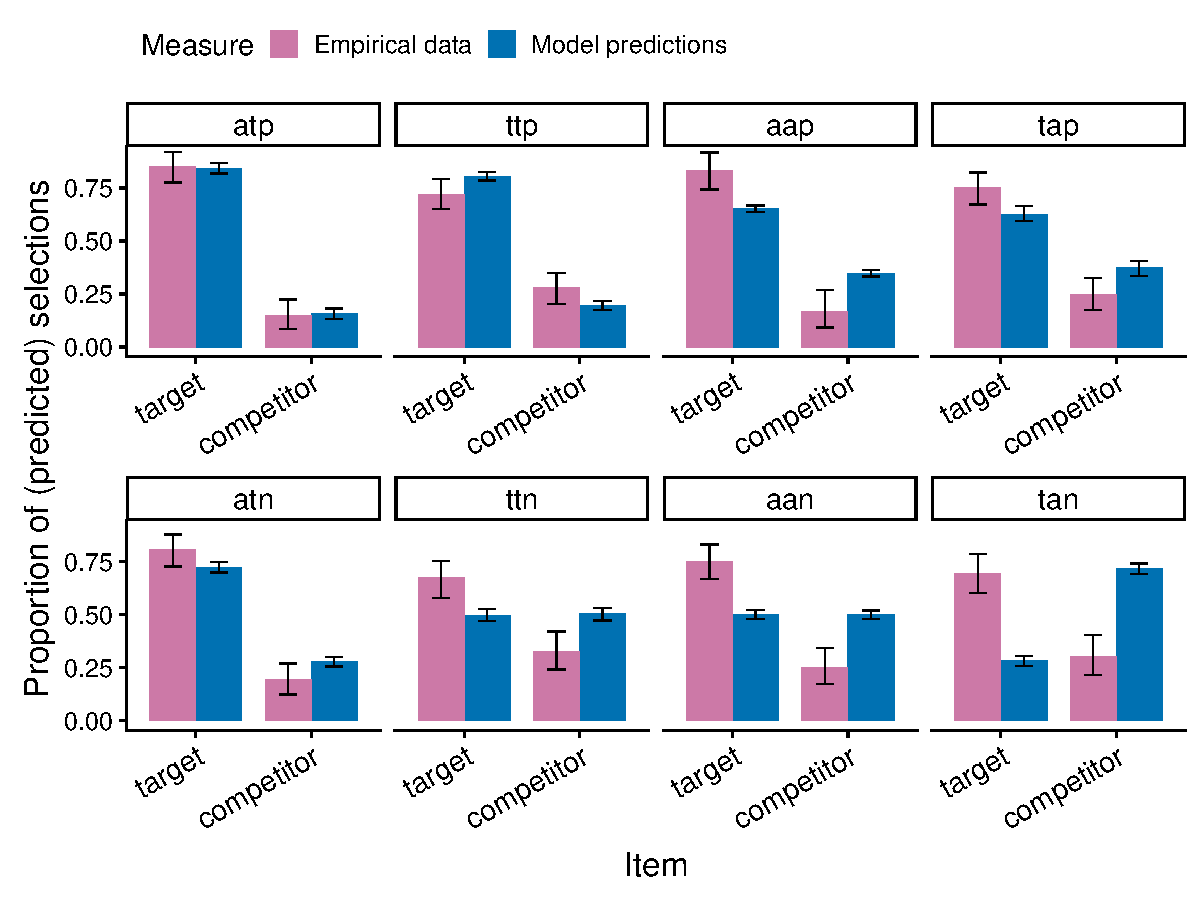
\includegraphics[width=.475\textwidth]{graphs/modelflat-bycondition-targetprevClick.pdf}
	\end{center}
\caption{This is a figure.\ek{fix a lot}} 
\label{model-results-flatprior-targetprev}
\end{figure}

\begin{figure}
	\begin{center}
		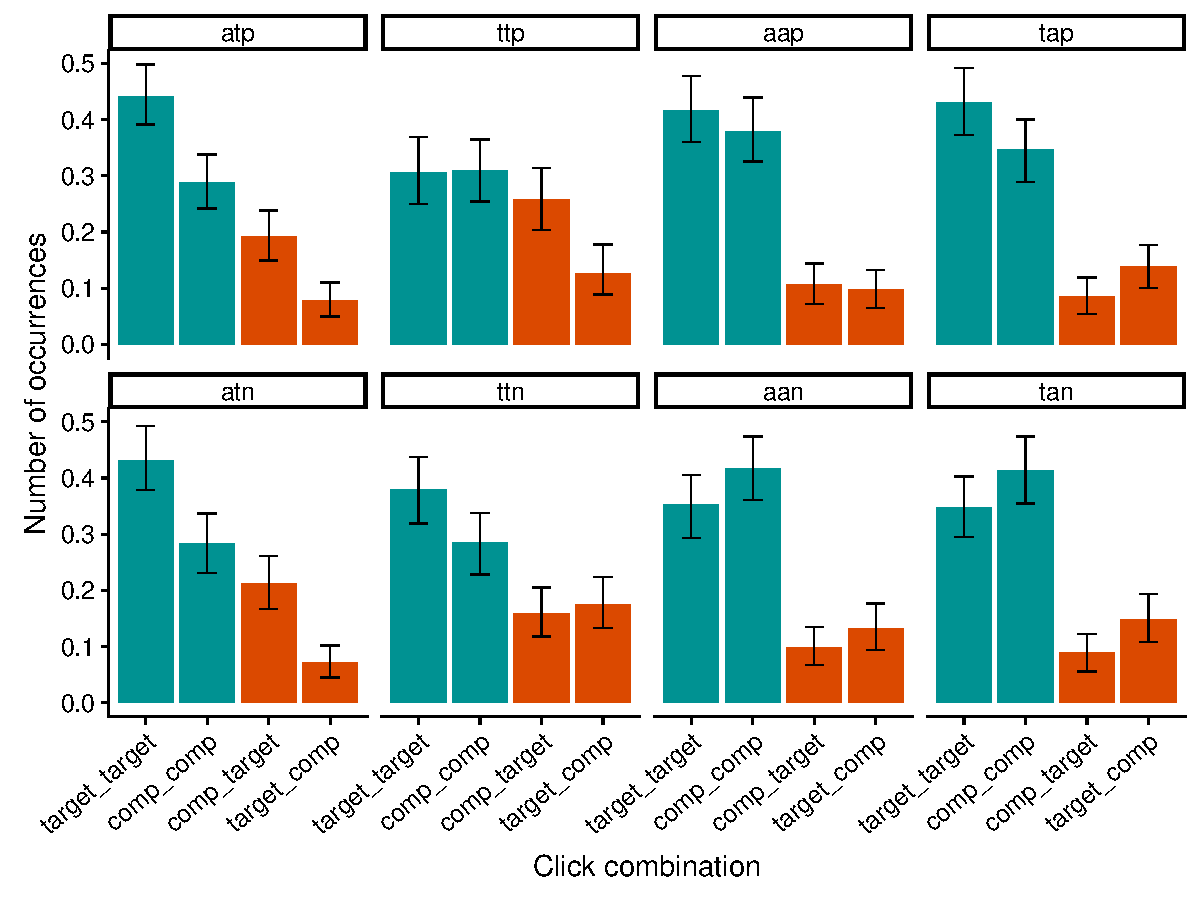
\includegraphics[width=.475\textwidth]{graphs/switching-bycond.pdf}
	\end{center}
\caption{This is a figure.\ek{fix a lot}} 
\label{switching}
\end{figure}



\section{Discussion}

\jd{somewhere make clear that it's not just color-diagnosticity of the target (as sedivy suggests) that matters -- instead, it's that, and the color-diagnosticity of the other distractors, and their relative typicality, etc etc, which are all ultimately captured variable modifier production expectations, and \emph{that's} the explanatory quantity}

\ek{random thought: if target is typical and contrast present -- does the typicality of the contrast affect modifier production for the target? It should. So far we see that modifier mention for the typical target + contrast contexts is not at ceiling, because (maybe) "banana" is still a better description of the target than the contrast. This would probably change if the contrast was brown.}

% There is not just a contrastive function on each adjective, but when a listener hears an adjective, it can be for multiple reasons, only one of which is contrastive. other reasons might be typicality, scene variation,... If we consider this to be true and the listener considers all objects in the display as potential targets, a lot of things need to be going alright for the target and competitor for the contrastive inference to happen. This also explains the difference between size and color adjectives, since size adjectives are not mentioned overinformatively.

% You can't take the results wrt presence/size of the contrastive inference effect and draw conclusions about the nature of adjective types. We can take color adjectives and make the contrastive inference (dis-)appear, i.e., we can make them look like size or material adjectives.

% We are showing that
% 1) listeners are highly pragmatic, i.e., they consider how well the utterance fits to each possible referent in the context and draws inferences about each and then takes them together -> competitor matters
% 2) thereby the modifier does not simply seem to receive a contrastive explanation for mentioning, but also a typicality explanation which affects the final inference just as much
% 3) taken together there simply seems to be an expectation of modifier inclusion which can result from multiple rationales.
% 4) we can make the contrastive inference strong (as for size adjectives) or disappear
% 5) in RSA we don't need to assume anything about the nature of the adjective, but can simply consider what the speaker probabilities for modifier use are... i.e., the linguistic knowledge can be obscure: we just need to consider production probabilities to predict listener behavior; underlyingly this could be simply communicative pressures; Due to informativity, the color needs to be mentioned if there is a contrast and the same holds for typicality (see PsychReview paper)






























% \section{General Formatting Instructions}

% The entire content of a paper (including figures, references, and anything else) can be no longer than six pages in the \textbf{initial submission}. In the \textbf{final submission}, the text of the paper, including an author line, must fit on six pages. Up to one additional page can be used for acknowledgements and references.

% The text of the paper should be formatted in two columns with an
% overall width of 7 inches (17.8 cm) and length of 9.25 inches (23.5
% cm), with 0.25 inches between the columns. Leave two line spaces
% between the last author listed and the text of the paper; the text of
% the paper (starting with the abstract) should begin no less than 2.75 inches below the top of the
% page. The left margin should be 0.75 inches and the top margin should
% be 1 inch.  \textbf{The right and bottom margins will depend on
%   whether you use U.S. letter or A4 paper, so you must be sure to
%   measure the width of the printed text.} Use 10~point Times Roman
% with 12~point vertical spacing, unless otherwise specified.

% The title should be in 14~point bold font, centered. The title should
% be formatted with initial caps (the first letter of content words
% capitalized and the rest lower case). In the initial submission, the
% phrase ``Anonymous CogSci submission'' should appear below the title,
% centered, in 11~point bold font.  In the final submission, each
% author's name should appear on a separate line, 11~point bold, and
% centered, with the author's email address in parentheses. Under each
% author's name list the author's affiliation and postal address in
% ordinary 10~point type.

% Indent the first line of each paragraph by 1/8~inch (except for the
% first paragraph of a new section). Do not add extra vertical space
% between paragraphs.


% \section{First Level Headings}

% First level headings should be in 12~point, initial caps, bold and
% centered. Leave one line space above the heading and 1/4~line space
% below the heading.


% \subsection{Second Level Headings}

% Second level headings should be 11~point, initial caps, bold, and
% flush left. Leave one line space above the heading and 1/4~line
% space below the heading.


% \subsubsection{Third Level Headings}

% Third level headings should be 10~point, initial caps, bold, and flush
% left. Leave one line space above the heading, but no space after the
% heading.


% \section{Formalities, Footnotes, and Floats}

% Use standard APA citation format. Citations within the text should
% include the author's last name and year. If the authors' names are
% included in the sentence, place only the year in parentheses, as in
% \citeA{NewellSimon1972a}, but otherwise place the entire reference in
% parentheses with the authors and year separated by a comma
% \cite{NewellSimon1972a}. List multiple references alphabetically and
% separate them by semicolons
% \cite{ChalnickBillman1988a,NewellSimon1972a}. Use the
% ``et~al.'' construction only after listing all the authors to a
% publication in an earlier reference and for citations with four or
% more authors.


% \subsection{Footnotes}

% Indicate footnotes with a number\footnote{Sample of the first
% footnote.} in the text. Place the footnotes in 9~point font at the
% bottom of the column on which they appear. Precede the footnote block
% with a horizontal rule.\footnote{Sample of the second footnote.}


% \subsection{Tables}

% Number tables consecutively. Place the table number and title (in
% 10~point) above the table with one line space above the caption and
% one line space below it, as in Table~\ref{sample-table}. You may float
% tables to the top or bottom of a column, and you may set wide tables across
% both columns.

% \begin{table}[H]
% \begin{center} 
% \caption{Sample table title.} 
% \label{sample-table} 
% \vskip 0.12in
% \begin{tabular}{ll} 
% \hline
% Error type    &  Example \\
% \hline
% Take smaller        &   63 - 44 = 21 \\
% Always borrow~~~~   &   96 - 42 = 34 \\
% 0 - N = N           &   70 - 47 = 37 \\
% 0 - N = 0           &   70 - 47 = 30 \\
% \hline
% \end{tabular} 
% \end{center} 
% \end{table}


% \subsection{Figures}

% All artwork must be very dark for purposes of reproduction and should
% not be hand drawn. Number figures sequentially, placing the figure
% number and caption, in 10~point, after the figure with one line space
% above the caption and one line space below it, as in
% Figure~\ref{sample-figure}. If necessary, leave extra white space at
% the bottom of the page to avoid splitting the figure and figure
% caption. You may float figures to the top or bottom of a column, and
% you may set wide figures across both columns.

% \begin{figure}[H]
% \begin{center}
% \fbox{CoGNiTiVe ScIeNcE}
% \end{center}
% \caption{This is a figure.} 
% \label{sample-figure}
% \end{figure}


% \section{Acknowledgments}

% In the \textbf{initial submission}, please \textbf{do not include
%   acknowledgements}, to preserve anonymity.  In the \textbf{final submission},
% place acknowledgments (including funding information) in a section \textbf{at
% the end of the paper}.


% \section{References Instructions}

% Follow the APA Publication Manual for citation format, both within the
% text and in the reference list, with the following exceptions: (a) do
% not cite the page numbers of any book, including chapters in edited
% volumes; (b) use the same format for unpublished references as for
% published ones. Alphabetize references by the surnames of the authors,
% with single author entries preceding multiple author entries. Order
% references by the same authors by the year of publication, with the
% earliest first.

% Use a first level section heading, ``{\bf References}'', as shown
% below. Use a hanging indent style, with the first line of the
% reference flush against the left margin and subsequent lines indented
% by 1/8~inch. Below are example references for a conference paper, book
% chapter, journal article, dissertation, book, technical report, and
% edited volume, respectively.

% \nocite{ChalnickBillman1988a}
% \nocite{Feigenbaum1963a}
% \nocite{Hill1983a}
% \nocite{OhlssonLangley1985a}
% % \nocite{Lewis1978a}
% \nocite{Matlock2001}
% \nocite{NewellSimon1972a}
% \nocite{ShragerLangley1990a}


\bibliographystyle{apacite}

\setlength{\bibleftmargin}{.125in}
\setlength{\bibindent}{-\bibleftmargin}

\bibliography{CogSci_Template}


\end{document}
